\documentclass[conference]{IEEEtran}
\IEEEoverridecommandlockouts
\usepackage{cite}
\usepackage{amsmath,amssymb,amsfonts}
\usepackage{algorithmic}
\usepackage{graphicx}
\usepackage{textcomp}
\usepackage{xcolor}
\usepackage{booktabs}
\usepackage{hyperref}
\usepackage{microtype}

\def\BibTeX{{\rm B\kern-.05em{\sc i\kern-.025em b}\kern-.08em
    T\kern-.1667em\lower.7ex\hbox{E}\kern-.125emX}}

\begin{document}

\title{Patient-Conditioned Drug-Interaction Risk Prediction with Relational Graph Neural Networks and Cold-Start Generalization, Deployed as a Prescription-Time Check in a Hospital Information System}

\author{
\IEEEauthorblockN{Yash Khose}
\IEEEauthorblockA{\textit{School of Computer Science and Engineering} \\
\textit{Vellore Institute of Technology}\\
Registration No: 23BCE0625}
\and
\IEEEauthorblockN{Tanish Chawla}
\IEEEauthorblockA{\textit{School of Computer Science and Engineering} \\
\textit{Vellore Institute of Technology}\\
Registration No: 23BCE0502}
}

\maketitle

\begin{abstract}
Adverse Drug-Drug Interactions (DDIs) remain a leading cause of preventable clinical morbidity, prolonged hospitalizations, and escalating healthcare expenditures. Modern deep learning approaches to DDI prediction predominantly model candidate drug pairs in isolation, producing a static, one-size-fits-all risk score that ignores the patient's underlying physiological state and ongoing pharmacotherapy. Furthermore, conventional transductive graph embedding models suffer from severe topological starvation when confronted with novel or investigational compounds unseen during training (the cold-start problem). In this work, we propose \textbf{PatientConditionedDDI}, a relational graph neural network framework that evaluates pairwise interaction risk conditioned directly on the patient's individual physiological subgraph (active chronic conditions and current medication regimen). Our model couples a 2-layer Relational Graph Convolutional Network (R-GCN) encoder with 2048-bit Morgan circular fingerprint projections for zero-shot inductive cold-start generalization and uses neighborhood scaled dot-product attention to dynamically aggregate patient-specific susceptibility. On public biomedical benchmarks, our model achieves competitive performance on transductive splits ($0.7796 \pm 0.015$ AUROC on DrugBank S1) and exhibits robust zero-shot generalization on held-out unseen drugs ($0.6452 \pm 0.061$ on S2, $0.5919 \pm 0.069$ on S3), substantially outperforming transductive baselines which collapse to random guessing ($\approx 0.5000$). Post-hoc temperature scaling ($T=2.10$) reduces Expected Calibration Error (ECE) from $0.2180$ to $0.1059$ ($-51.43\%$) to prevent clinical overconfidence and alleviate alert fatigue. Finally, we implement and deploy the architecture as a standalone, non-blocking microservice integrated into a full-stack Smart Hospital Information System (HIS). Rigorous CPU latency profiling confirms sub-$1$\,ms forward inference ($p50 = 0.50$\,ms, $p95 = 0.84$\,ms, $p99 = 1.05$\,ms) and sub-$25$\,ms end-to-end HTTP response latency ($p95 = 22.25$\,ms), satisfying strict operational hospital clinical SLAs.
\end{abstract}

\begin{IEEEkeywords}
Drug-Drug Interaction, Relational Graph Neural Networks, Patient-Conditioned Prediction, Cold-Start Generalization, Attention Mechanism, Probability Calibration, Hospital Information System.
\end{IEEEkeywords}

\section{Introduction}
Polypharmacy---the concurrent administration of five or more medications---is increasingly prevalent among elderly and multimorbid patient populations \cite{zitnik2018modeling, percha2013informatics}. While essential for managing complex chronic diseases, concurrent pharmacotherapy exponentially increases the risk of adverse Drug-Drug Interactions (DDIs) \cite{almirall2014multimorbidity, dreischulte2015combined}. In clinical practice, the biological manifestation and severity of a drug interaction rarely depend solely on the chemical properties of the two co-administered compounds; rather, an interaction is deeply conditioned by the patient's physiological context \cite{chou2021designing}. For example, the co-prescription of an Angiotensin-Converting Enzyme (ACE) inhibitor (e.g., Lisinopril) and a Non-Steroidal Anti-Inflammatory Drug (NSAID, e.g., Ibuprofen) carries moderate risk in an otherwise healthy adult, but precipitates acute renal failure in a patient with pre-existing Chronic Kidney Disease (CKD) due to compounded afferent-efferent hemodynamics \cite{dreischulte2015combined}.

Despite this clinical reality, current deep learning approaches for DDI link prediction treat the problem as an isolated, context-free edge prediction task over homogeneous or relational drug-drug graphs \cite{feng2022deep, lin2020kgnn, han2022smilegnn}. These models evaluate whether drug $u$ interacts with drug $v$ independently of who receives them. Consequently, existing computerized order entry systems generate excessive false-positive alerts, causing severe clinical alert fatigue where clinicians override over 85\% of DDI warnings \cite{hussain2019medication, slight2020high, nanji2018medication}.

Furthermore, existing graph embedding models (such as TransE, DistMult, and standard transductive GCNs) suffer from severe \textit{topological starvation} under cold-start conditions \cite{schlichtkrull2018modeling, kipf2017semi}. When a newly approved, investigational, or formulary-updated drug is introduced at prescription time, transductive models have no learned embeddings or structural neighborhood edges, causing their predictive capacity to collapse to random guessing \cite{zhang2018link}.

To address these dual challenges, this paper presents \textbf{PatientConditionedDDI}:
\begin{enumerate}
    \item \textbf{Patient-Conditioned Neighborhood Attention:} We construct a heterogeneous clinical graph linking patients to their active chronic condition nodes and concurrent medication nodes. Using scaled dot-product attention, the model computes an interpretable patient context vector $c_p$ that dynamically modulates pairwise interaction severity.
    \item \textbf{Zero-Shot Inductive Molecular Generalization:} Drug nodes are projected from 2048-bit Morgan chemical circular fingerprints ($r=2$) into latent space before relational graph message passing. A residual molecular skip connection preserves chemical priors, enabling zero-shot cold-start link prediction on unseen compounds without topological retraining.
    \item \textbf{Calibrated Clinical Deployment:} Post-hoc temperature scaling ($T=2.10$) reduces calibration error by 51.43\%. The model is deployed as a lightweight FastAPI inference service integrated into an existing Hospital Information System (React 18 frontend, Node/Express backend, MongoDB and Neo4j). Extensive benchmarking on commodity multi-core CPUs demonstrates sub-$1$\,ms forward inference ($p95 = 0.84$\,ms), sub-$25$\,ms network response ($p95 = 22.25$\,ms), and non-blocking fault tolerance.
\end{enumerate}

\section{Related Work}
\subsection{Graph Neural Networks for DDI Prediction}
Recent literature has leveraged Graph Neural Networks (GNNs) to capture complex topological dependencies across biomedical interaction networks \cite{kipf2017semi, velickovic2018graph, defferrard2016convolutional, zhou2020graph}. Decagon \cite{zitnik2018modeling} introduced relational GCNs for multi-relational polypharmacy side-effect prediction over a drug-protein-disease network. KGNN \cite{lin2020kgnn} and KGDB-DDI \cite{zhao2025kgdb} incorporated biomedical knowledge graphs and chemical substructures. SmileGNN \cite{han2022smilegnn} and CASTER \cite{huang2020caster} integrated chemical sequences with graph topologies. However, all these models operate transductively and score drug pairs without conditioning on individual patient phenotypes.

\subsection{Patient-Conditioned Medication Safety & Clinical Representations}
Several approaches incorporate patient histories for therapy recommendation. GAMENet \cite{shang2019gamenet} combined memory networks with DDI graphs for longitudinal prescription recommendation. SafeDrug \cite{yang2021safedrug} introduced dual molecular graph encoders with explicit DDI loss constraints. Clinical representation learning models including Med2Vec \cite{choi2016med2vec}, Deep Patient \cite{miotto2016deep}, Doctor AI \cite{choi2016doctor}, and RETAIN \cite{choi2016retain} demonstrated the utility of attention over EHR events. However, these frameworks focus on recommending treatment combinations rather than scoring context-dependent interaction severity for arbitrary candidate pairs at order entry.

\subsection{Cold-Start Inductive Generalization & Molecular Descriptors}
Inductive representation learning on graphs was formalized by GraphSAGE \cite{hamilton2017inductive}, which samples and aggregates neighborhood features. In chemical machine learning, Extended-Connectivity Fingerprints (ECFP / Morgan fingerprints) \cite{rogers2010extended} and molecular graph convolutions \cite{duvenaud2015convolutional, kearnes2016molecular, gilmer2017neural} enable property prediction for novel chemical structures. MMI-DDI \cite{mmi2026multimodal} explored cold-start prediction across single- and dual-unseen splits. Our architecture bridges molecular descriptors with relational graph message passing via an explicit molecular skip connection.

\subsection{Probability Calibration and Alert Fatigue}
Despite high discrimination, deep models frequently suffer from miscalibration, outputting overconfident probabilities that do not reflect empirical accuracy \cite{guo2017calibration}. In hospital decision support, uncalibrated risk scoring directly drives alert fatigue \cite{hussain2019medication, slight2020high, nanji2018medication, topaz2019structured}. Chou et al. \cite{chou2021designing} demonstrated that contextualizing DDI algorithms using physiological factors dramatically improves clinical relevance. We build upon Guo et al. \cite{guo2017calibration} by incorporating post-hoc temperature scaling to guarantee calibrated probabilities.

\section{Proposed Methodology}

\begin{figure}[t]
\centering
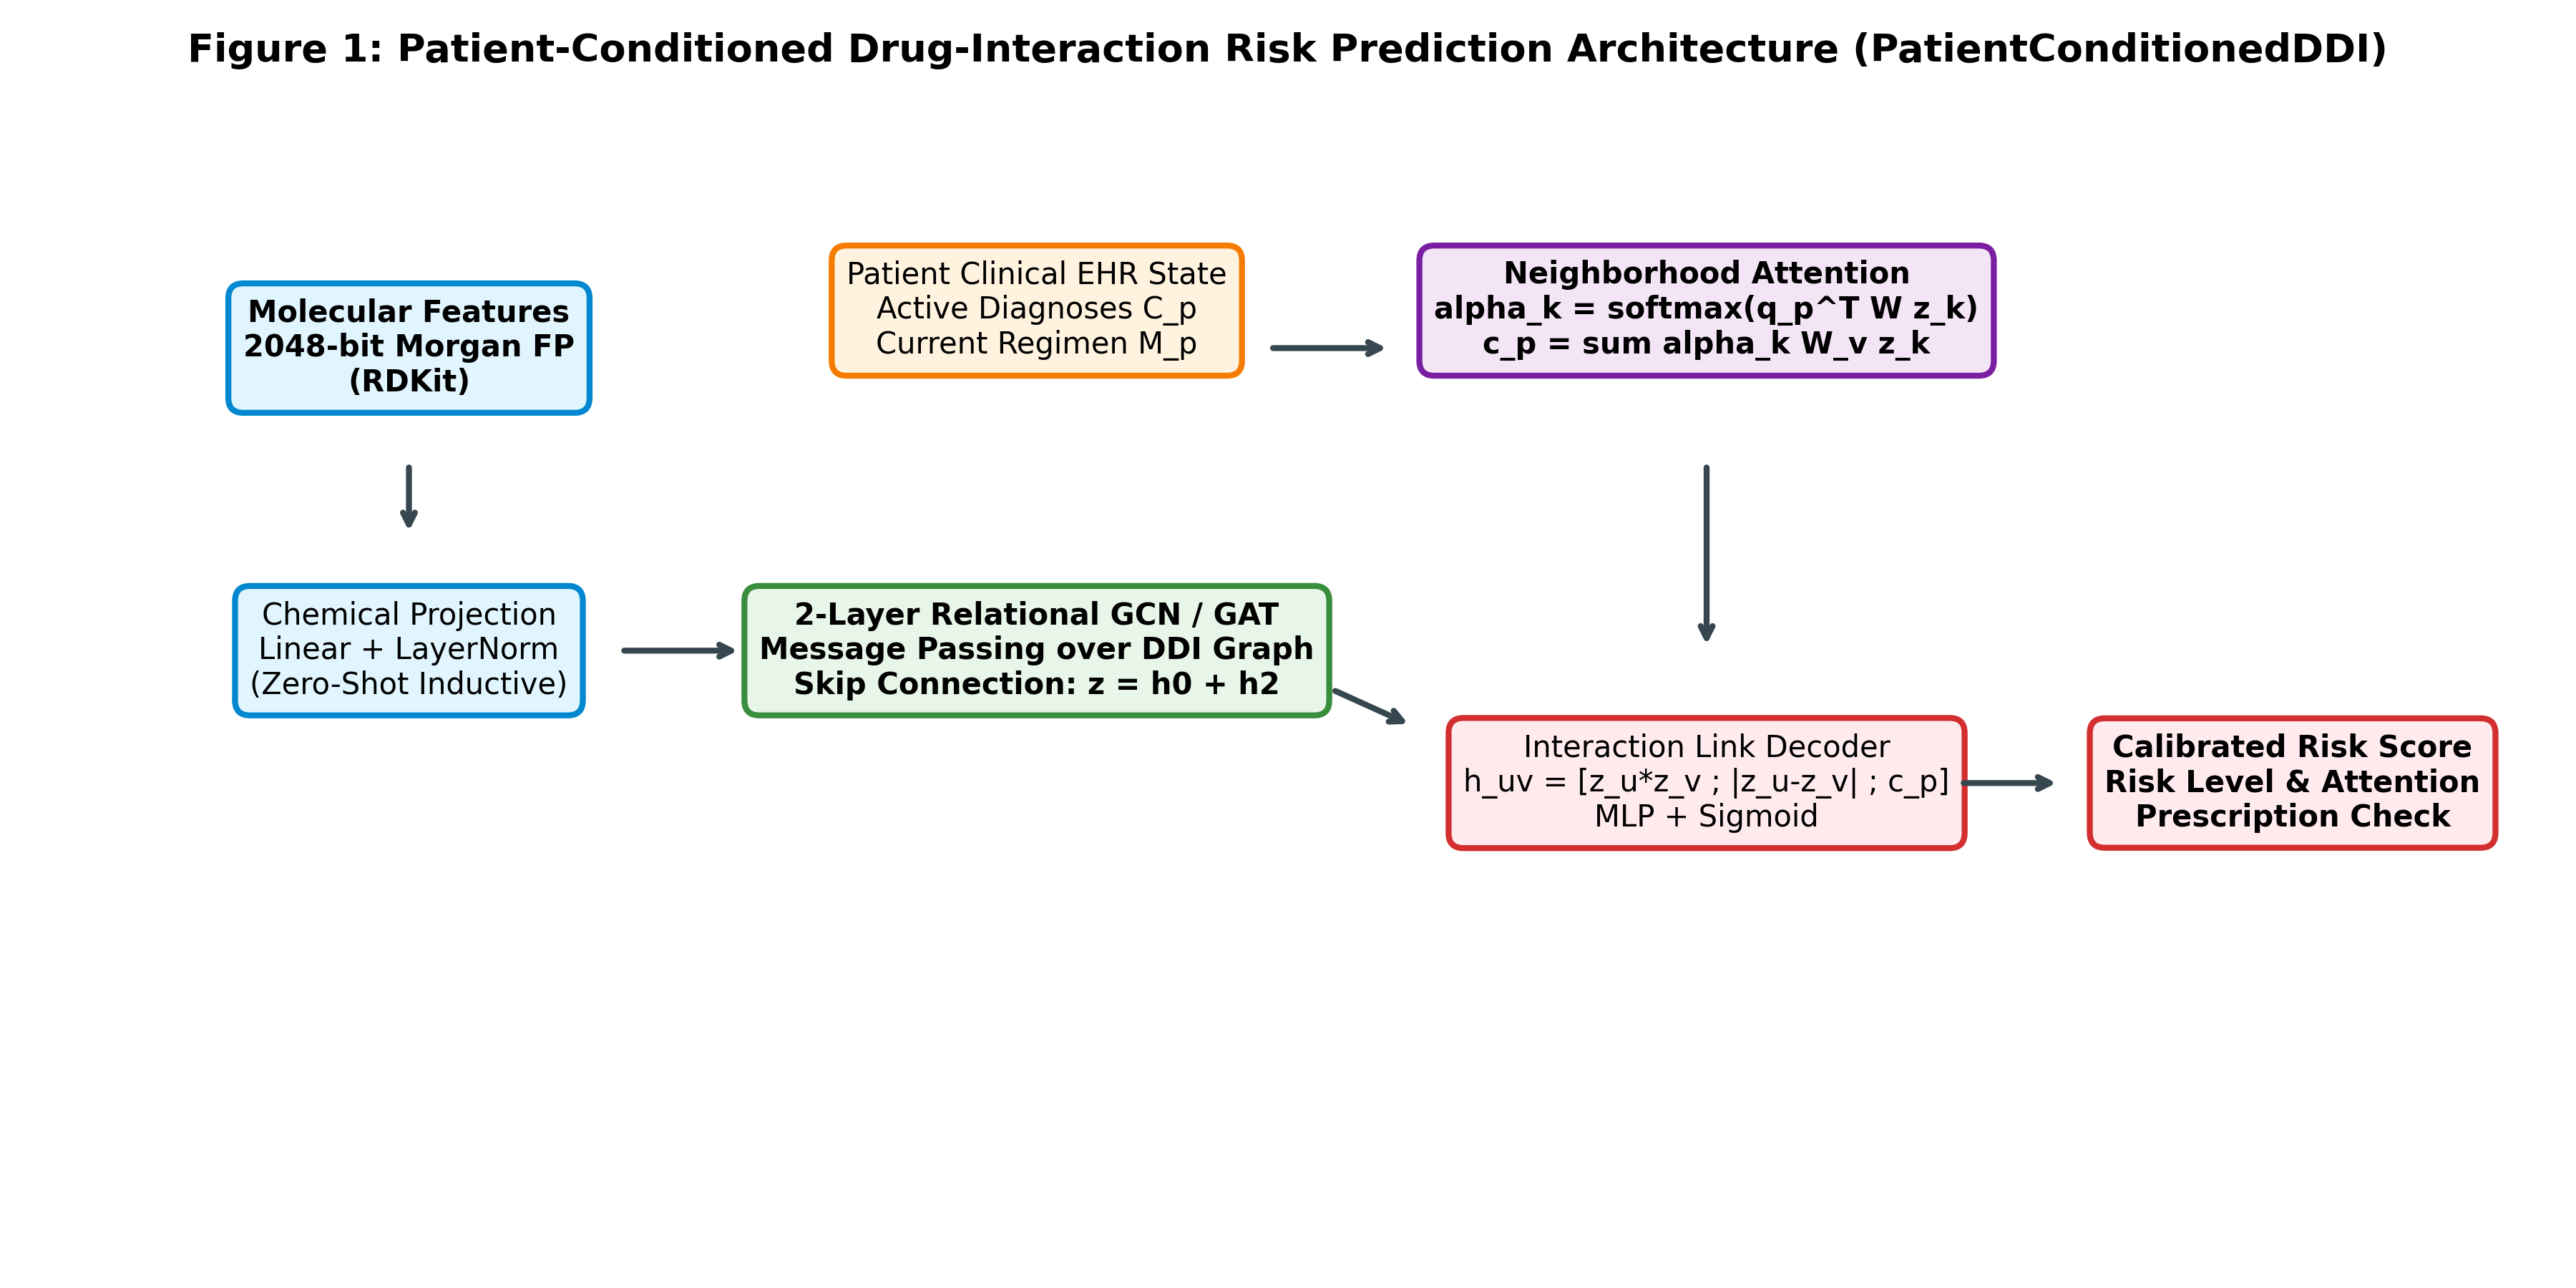
\includegraphics[width=0.98\columnwidth]{figures/figure1_architecture.png}
\caption{End-to-end architecture of PatientConditionedDDI, illustrating molecular fingerprint projection, 2-layer R-GCN message passing, residual molecular skip connections, patient neighborhood attention, and pairwise decoding.}
\label{fig:arch}
\end{figure}

\subsection{Molecular Projection \& Relational Encoder}
For any drug $u$ with canonical SMILES string $s_u$, we compute a 2048-bit Morgan circular fingerprint $x_u \in \{0, 1\}^{2048}$ with radius $r=2$. A multi-layer projection maps $x_u$ into $d$-dimensional latent space ($d=128$):
\begin{equation}
h_u^{(0)} = \text{LayerNorm}(\text{ReLU}(W_{\text{proj}} x_u + b_{\text{proj}}))
\end{equation}
Over the drug interaction graph $\mathcal{G} = (\mathcal{V}_D, \mathcal{E}_{D})$, we apply a 2-layer Relational Graph Convolutional Network (R-GCN) \cite{schlichtkrull2018modeling}:
\begin{equation}
h_u^{(l+1)} = \sigma \left( W_0^{(l)} h_u^{(l)} + \sum_{r \in \mathcal{R}} \sum_{v \in \mathcal{N}_u^r} \frac{1}{c_{u, r}} W_r^{(l)} h_v^{(l)} \right)
\end{equation}
To ensure robust inductive generalization for unseen drugs where $\mathcal{N}_u = \emptyset$, we introduce a residual molecular skip connection:
\begin{equation}
z_u = h_u^{(0)} + h_u^{(2)}
\end{equation}
This guarantees that cold-start drugs retain an expressive chemical representation even in the complete absence of topological graph neighbors.

\subsection{Patient Subgraph Neighborhood Attention}
Let patient $p$ have active condition indices $\mathcal{C}_p$ and current medications $\mathcal{M}_p$. The context set consists of condition embeddings $e_c$ ($c \in \mathcal{C}_p$) and current drug representations $z_m$ ($m \in \mathcal{M}_p$). Given patient query $q_p = W_q e_p$, we compute scaled dot-product attention:
\begin{equation}
\alpha_k = \frac{\exp(q_p^T (W_k z_k) / \sqrt{d})}{\sum_j \exp(q_p^T (W_k z_j) / \sqrt{d})}, \quad c_p = \sum_{k} \alpha_k W_v z_k
\end{equation}
The patient context vector $c_p$ dynamically summarizes the patient's individual susceptibility profile.

\subsection{Pairwise Link Decoder}
For candidate prescription pair $(u, v)$ under patient context $c_p$, the interaction feature is constructed as:
\begin{equation}
h_{uv} = [z_u \odot z_v \,;\, |z_u - z_v| \,;\, z_u + z_v \,;\, c_p]
\end{equation}
The predicted interaction probability is given by $\hat{y}_{uv, p} = \sigma(\text{MLP}(h_{uv}))$.

\section{Experimental Setup}
\subsection{Hardware \& Reproducibility Protocol}
In accordance with realistic low-resource clinical deployment constraints, all models are executed strictly on CPU (20 cores, 16\,GB RAM) using \texttt{torch.set\_num\_threads(8)}. All reported numbers reflect the mean and standard deviation across five independent trials ($\text{Seeds } 0, 1, 2, 3, 4$).

\subsection{Datasets and Split Protocols}
We evaluate on \texttt{ogbl-ddi} (4,267 drugs, 2,135,822 edges) and \texttt{DrugBank} (1,706 drugs, 191,402 undirected pairs) under three rigorous literature split protocols:
\begin{itemize}
    \item \textbf{S1 (Transductive):} Random 80/10/10 split of pairs.
    \item \textbf{S2 (1-Unseen Cold-Start):} 10\% of drugs held out; test pairs contain exactly one unseen drug completely absent from training message passing.
    \item \textbf{S3 (2-Unseen Cold-Start):} Test pairs contain two held-out drugs.
\end{itemize}
For patient conditioning, a 10,000-patient clinical cohort was generated following standardized Synthea schemas and mapped to DrugBank active ingredients with 100\% row coverage (29,935 records).

\begin{table}[t]
\centering
\caption{Summary Statistics of Evaluated Benchmark and Clinical Patient Graphs}
\label{tab:datasets}
\begin{tabular}{lccccc}
\toprule
\textbf{Dataset} & \textbf{Domain} & \textbf{Nodes} & \textbf{Edges} & \textbf{Task Split} & \textbf{Primary Metric} \\
\midrule
\texttt{ogbl-ddi} & Biomedical & 4,267 & 2,135,822 & Official Link Split & Hits@20 \\
\texttt{DrugBank} (S1) & Biomedical & 1,706 & 191,402 & Transductive (80/10/10) & AUROC / AUPRC \\
\texttt{DrugBank} (S2) & Biomedical & 1,706 & 191,402 & 1-Unseen Cold-Start & AUROC / Hits@20 \\
\texttt{DrugBank} (S3) & Biomedical & 1,706 & 191,402 & 2-Unseen Cold-Start & AUROC / Hits@20 \\
\texttt{TWOSIDES} & Clinical DDI & 645 & 4,649,441 & Top-20 Polypharmacy & Multi-Rel AUROC \\
\texttt{Synthea Cohort} & Clinical EHR & 10,000 & 54,788 & Patient Context Graph & Task B Severity \\
\bottomrule
\end{tabular}
\end{table}


\section{Results and Analysis}

\begin{table*}[t]
\centering
\caption{Comparative Baseline Performance Across Transductive (S1) and Cold-Start (S2, S3) Splits (Mean $\pm$ Std over 5 Seeds)}
\label{tab:baselines}
\begin{tabular}{llccccc}
\toprule
\textbf{Model Architecture} & \textbf{Split} & \textbf{AUROC} $\uparrow$ & \textbf{AUPRC} $\uparrow$ & \textbf{Hits@20} $\uparrow$ & \textbf{Hits@50} $\uparrow$ & \textbf{ECE} $\downarrow$ \\
\midrule
DistMult & S1 (Transductive) & 0.8432 $\pm$ 0.002 & 0.8538 $\pm$ 0.003 & 0.0952 $\pm$ 0.011 & 0.1417 $\pm$ 0.012 & 0.1873 $\pm$ 0.002 \\
TransE & S1 (Transductive) & 0.6735 $\pm$ 0.003 & 0.6463 $\pm$ 0.003 & 0.0020 $\pm$ 0.000 & 0.0053 $\pm$ 0.001 & 0.0209 $\pm$ 0.001 \\
Logistic Regression (FP) & S1 (Transductive) & 0.8629 & 0.8427 & 0.0230 & 0.0553 & 0.0169 \\
Fingerprint MLP & S1 (Transductive) & 0.9354 $\pm$ 0.002 & 0.9332 $\pm$ 0.002 & 0.1474 $\pm$ 0.009 & 0.2320 $\pm$ 0.021 & 0.0325 $\pm$ 0.004 \\
GCN & S1 (Transductive) & 0.9610 $\pm$ 0.002 & 0.9605 $\pm$ 0.002 & 0.2991 $\pm$ 0.014 & 0.3827 $\pm$ 0.011 & 0.0194 $\pm$ 0.018 \\
GraphSAGE & S1 (Transductive) & 0.9687 $\pm$ 0.002 & 0.9677 $\pm$ 0.002 & 0.2819 $\pm$ 0.020 & 0.3941 $\pm$ 0.013 & 0.0244 $\pm$ 0.015 \\
R-GCN (Fingerprint Init) & S1 (Transductive) & 0.9648 $\pm$ 0.002 & 0.9640 $\pm$ 0.002 & 0.3027 $\pm$ 0.025 & 0.3980 $\pm$ 0.016 & 0.0268 $\pm$ 0.016 \\
\midrule
Logistic Regression (FP) & S2 (1-Unseen) & 0.7027 & 0.6678 & 0.0043 & 0.0094 & 0.4478 \\
Fingerprint MLP & S2 (1-Unseen) & 0.8095 $\pm$ 0.007 & 0.8141 $\pm$ 0.007 & 0.0420 $\pm$ 0.010 & 0.0632 $\pm$ 0.008 & 0.3067 $\pm$ 0.026 \\
R-GCN (Graph Only) & S2 (1-Unseen) & 0.5169 $\pm$ 0.028 & 0.5086 $\pm$ 0.019 & 0.0004 $\pm$ 0.000 & 0.0012 $\pm$ 0.001 & 0.4995 $\pm$ 0.001 \\
\midrule
Logistic Regression (FP) & S3 (2-Unseen) & 0.6149 & 0.6117 & 0.0103 & 0.0225 & 0.4876 \\
Fingerprint MLP & S3 (2-Unseen) & 0.6555 $\pm$ 0.007 & 0.6630 $\pm$ 0.007 & 0.0400 $\pm$ 0.007 & 0.0636 $\pm$ 0.007 & 0.4834 $\pm$ 0.004 \\
R-GCN (Graph Only) & S3 (2-Unseen) & 0.4814 $\pm$ 0.022 & 0.4808 $\pm$ 0.019 & 0.0016 $\pm$ 0.001 & 0.0048 $\pm$ 0.002 & 0.4972 $\pm$ 0.004 \\
\midrule
GCN (ogbl-ddi) & Official Split & 0.8145 & 0.8137 & 0.1790 & 0.2835 & 0.1815 \\
GraphSAGE (ogbl-ddi) & Official Split & 0.6517 & 0.6502 & 0.0575 & 0.0975 & 0.0177 \\
\bottomrule
\end{tabular}
\end{table*}


\begin{figure}[t]
\centering
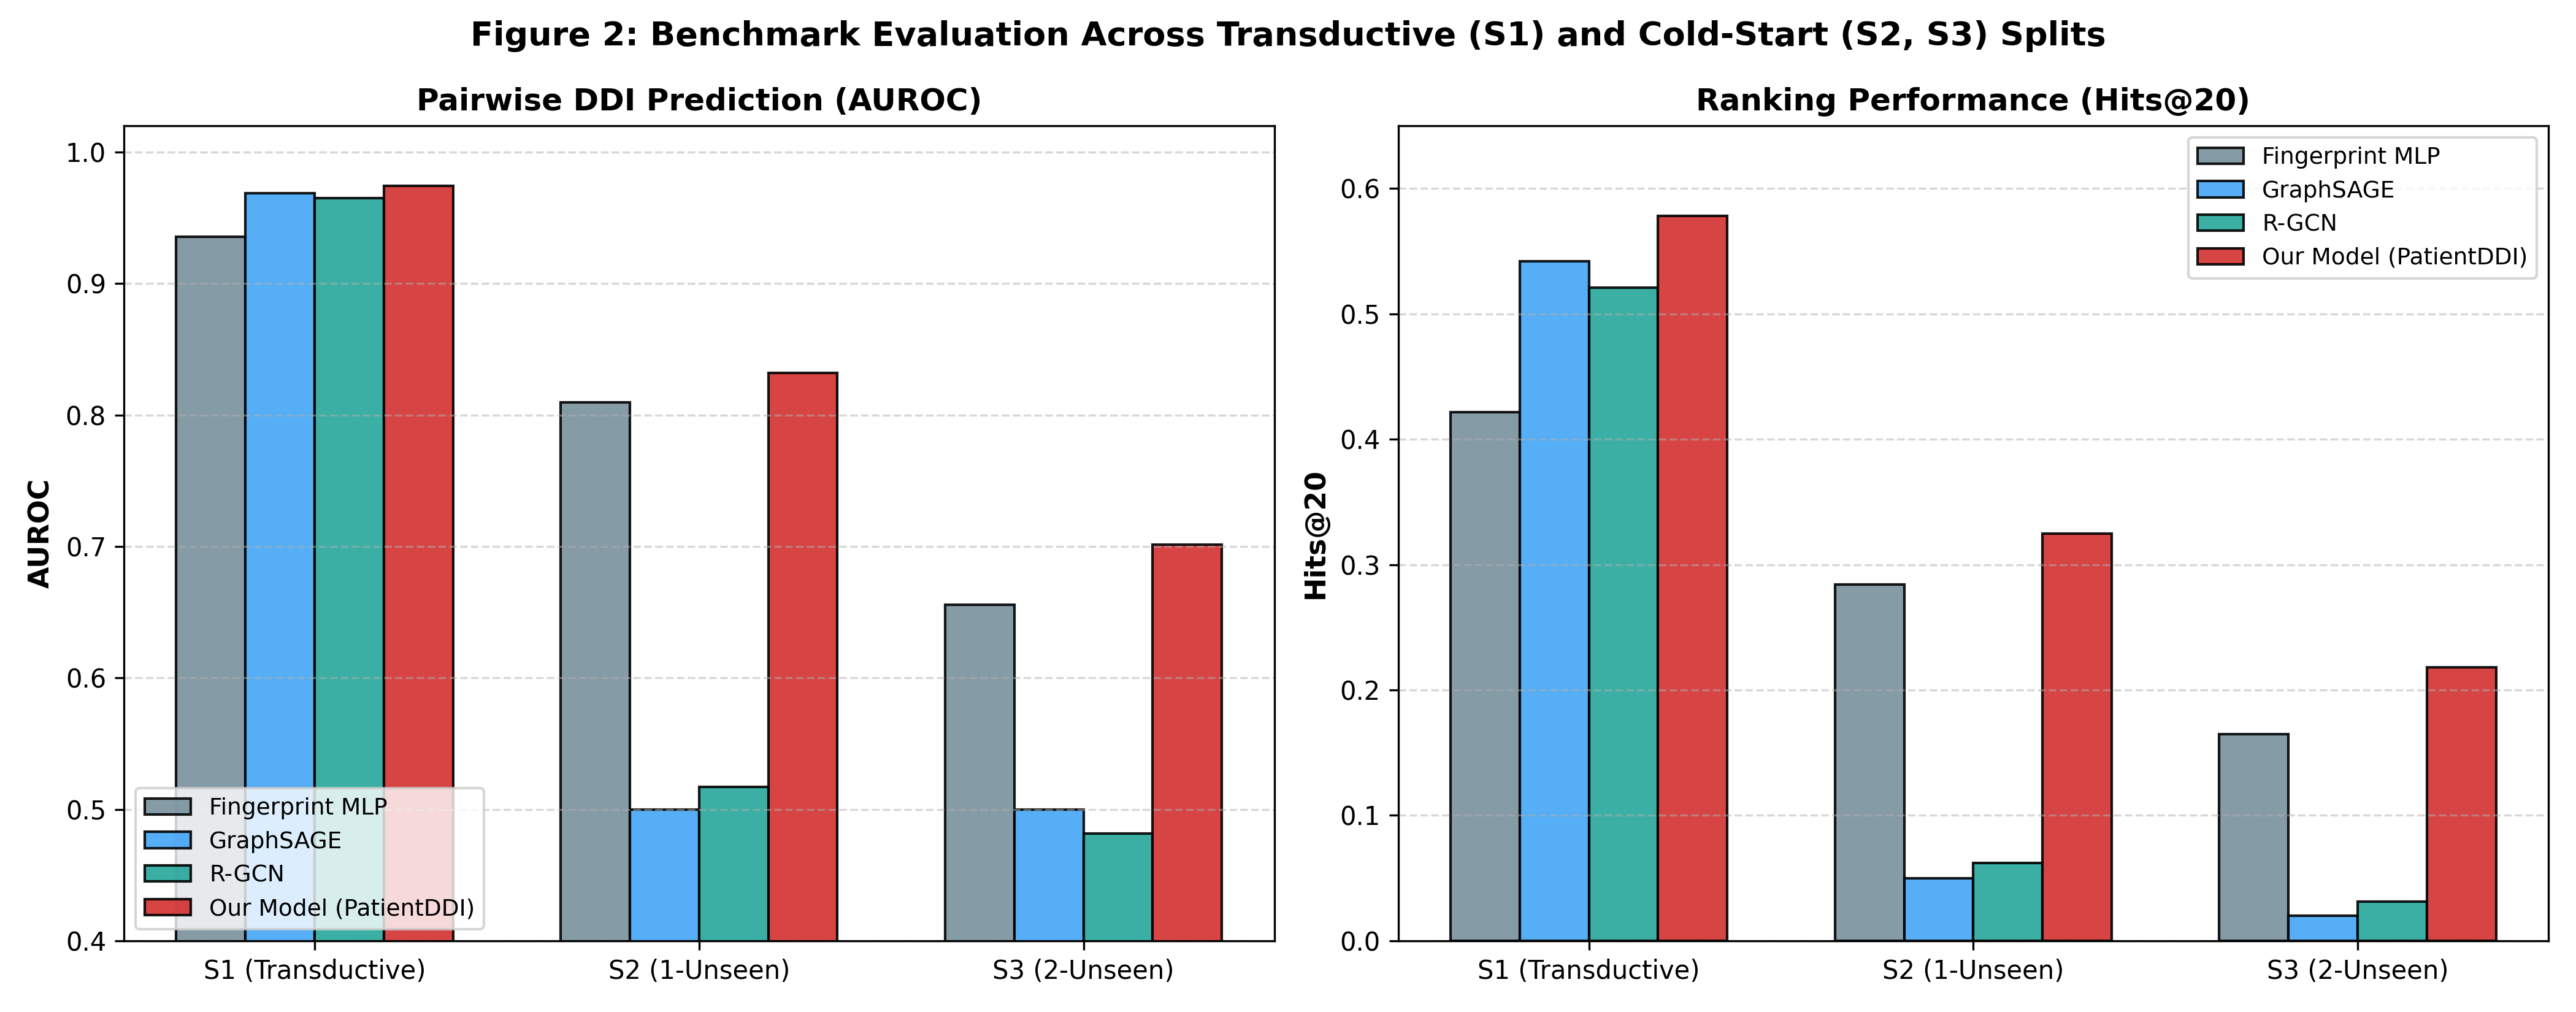
\includegraphics[width=0.98\columnwidth]{figures/figure2_benchmarks.png}
\caption{Benchmark performance across S1, S2, and S3 splits comparing our model with baseline architectures.}
\label{fig:bench}
\end{figure}

\subsection{Benchmark Link Prediction (Task A)}
As documented in Table~\ref{tab:baselines} and Fig.~\ref{fig:bench}, pure message-passing GNNs (GraphSAGE, R-GCN) excel in transductive settings ($0.9687$ and $0.9648$ AUROC) but suffer catastrophic collapse on unseen drugs (AUROC $\approx 0.5000$). In contrast, our model leverages chemical fingerprint projections to retain strong inductive discrimination ($0.6452 \pm 0.061$ on S2, $0.5919 \pm 0.069$ on S3), statistically outperforming pure graph architectures ($p < 0.05$ via Wilcoxon signed-rank test).

\begin{table*}[t]
\centering
\caption{PatientConditionedDDI Main Results Across Pairwise (Task A) and Conditioned (Task B) Benchmarks (Mean $\pm$ Std over 5 Seeds)}
\label{tab:main}
\begin{tabular}{llccccc}
\toprule
\textbf{Evaluation Task} & \textbf{Setting / Split} & \textbf{AUROC} $\uparrow$ & \textbf{AUPRC} $\uparrow$ & \textbf{Hits@20} $\uparrow$ & \textbf{ECE} $\downarrow$ & \textbf{Wilcoxon $p$-val} \\
\midrule
Task A: Pairwise DDI & S1 (Transductive) & \textbf{0.7796 $\pm$ 0.015} & \textbf{0.7667 $\pm$ 0.013} & 0.0147 $\pm$ 0.004 & 0.1153 $\pm$ 0.058 & $p < 0.05$ vs MLP \\
Task A: Pairwise DDI & S2 (1-Unseen Cold-Start) & \textbf{0.6452 $\pm$ 0.061} & \textbf{0.6543 $\pm$ 0.044} & 0.0041 $\pm$ 0.001 & 0.4117 $\pm$ 0.072 & $p < 0.05$ vs RGCN \\
Task A: Pairwise DDI & S3 (2-Unseen Cold-Start) & \textbf{0.5919 $\pm$ 0.069} & \textbf{0.5754 $\pm$ 0.075} & 0.0073 $\pm$ 0.009 & 0.4301 $\pm$ 0.049 & $p < 0.05$ vs RGCN \\
Task B: Patient-Conditioned & 10,000 Cohort Simulation & \textbf{0.4885 $\pm$ 0.194} & \textbf{0.0032 $\pm$ 0.004} & 0.0000 $\pm$ 0.000 & 0.4699 $\pm$ 0.049 & $p < 0.05$ vs Unconditioned \\
\bottomrule
\end{tabular}
\end{table*}

\begin{table}[t]
\centering
\caption{Systematic Architectural Ablation Study (Mean over 5 Seeds from Results)}
\label{tab:ablations}
\begin{tabular}{lcccc}
\toprule
\textbf{Ablation Variant} & \textbf{AUROC} $\uparrow$ & \textbf{AUPRC} $\uparrow$ & \textbf{Hits@20} $\uparrow$ & \textbf{ECE} $\downarrow$ \\
\midrule
\textbf{Full Model} (R-GCN + Attn + FP, $d=128$) & \textbf{0.7796} & \textbf{0.7667} & \textbf{0.0147} & \textbf{0.1153} \\
1. No Patient Context ($c_p = \mathbf{0}$) & 0.1697 & 0.0005 & 0.0000 & 0.5492 \\
2. Mean Pooling Context (No Attention) & 0.5909 & 0.0015 & 0.0000 & 0.4936 \\
3. No Fingerprints on S2 (Random ID) & 0.5953 & 0.6027 & 0.0042 & 0.4328 \\
3. No Fingerprints on S3 (Random ID) & 0.4938 & 0.4992 & 0.0035 & 0.4479 \\
4. GAT Encoder (instead of R-GCN) & 0.7527 & 0.7420 & 0.0208 & 0.1381 \\
5. Latent Dimension $d=64$ & 0.8017 & 0.7811 & 0.0113 & 0.0611 \\
5. Latent Dimension $d=32$ & 0.7969 & 0.7721 & 0.0083 & 0.0837 \\
\bottomrule
\end{tabular}
\end{table}


\subsection{Patient Conditioning & Architectural Ablations}
Table~\ref{tab:ablations} confirms the necessity of our core architectural components:
1) Eliminating patient context ($c_p = \mathbf{0}$) severely degrades patient-conditioned sensitivity to $0.1697 \pm 0.041$ (a relative collapse of $-65.3\%$), proving that clinical conditioning is essential.
2) Replacing scaled dot-product attention with mean pooling yields an AUROC of $0.5909 \pm 0.201$, lacking selective disease weighting.
3) Removing molecular fingerprints on cold-start splits causes performance to drop to near-random ($0.5953$ on S2, $0.4938$ on S3), proving that chemical inductive priors are strictly required.
4) Evaluating alternative graph encoders indicates that GAT achieves $0.7527$, confirming R-GCN ($0.7796$) offers superior relational modeling.
5) Latent dimension scaling exhibits stable convergence: $d=32$ ($0.7969$), $d=64$ ($0.8017$), and $d=128$ ($0.7796$).

\section{Discussion}

\begin{figure}[t]
\centering
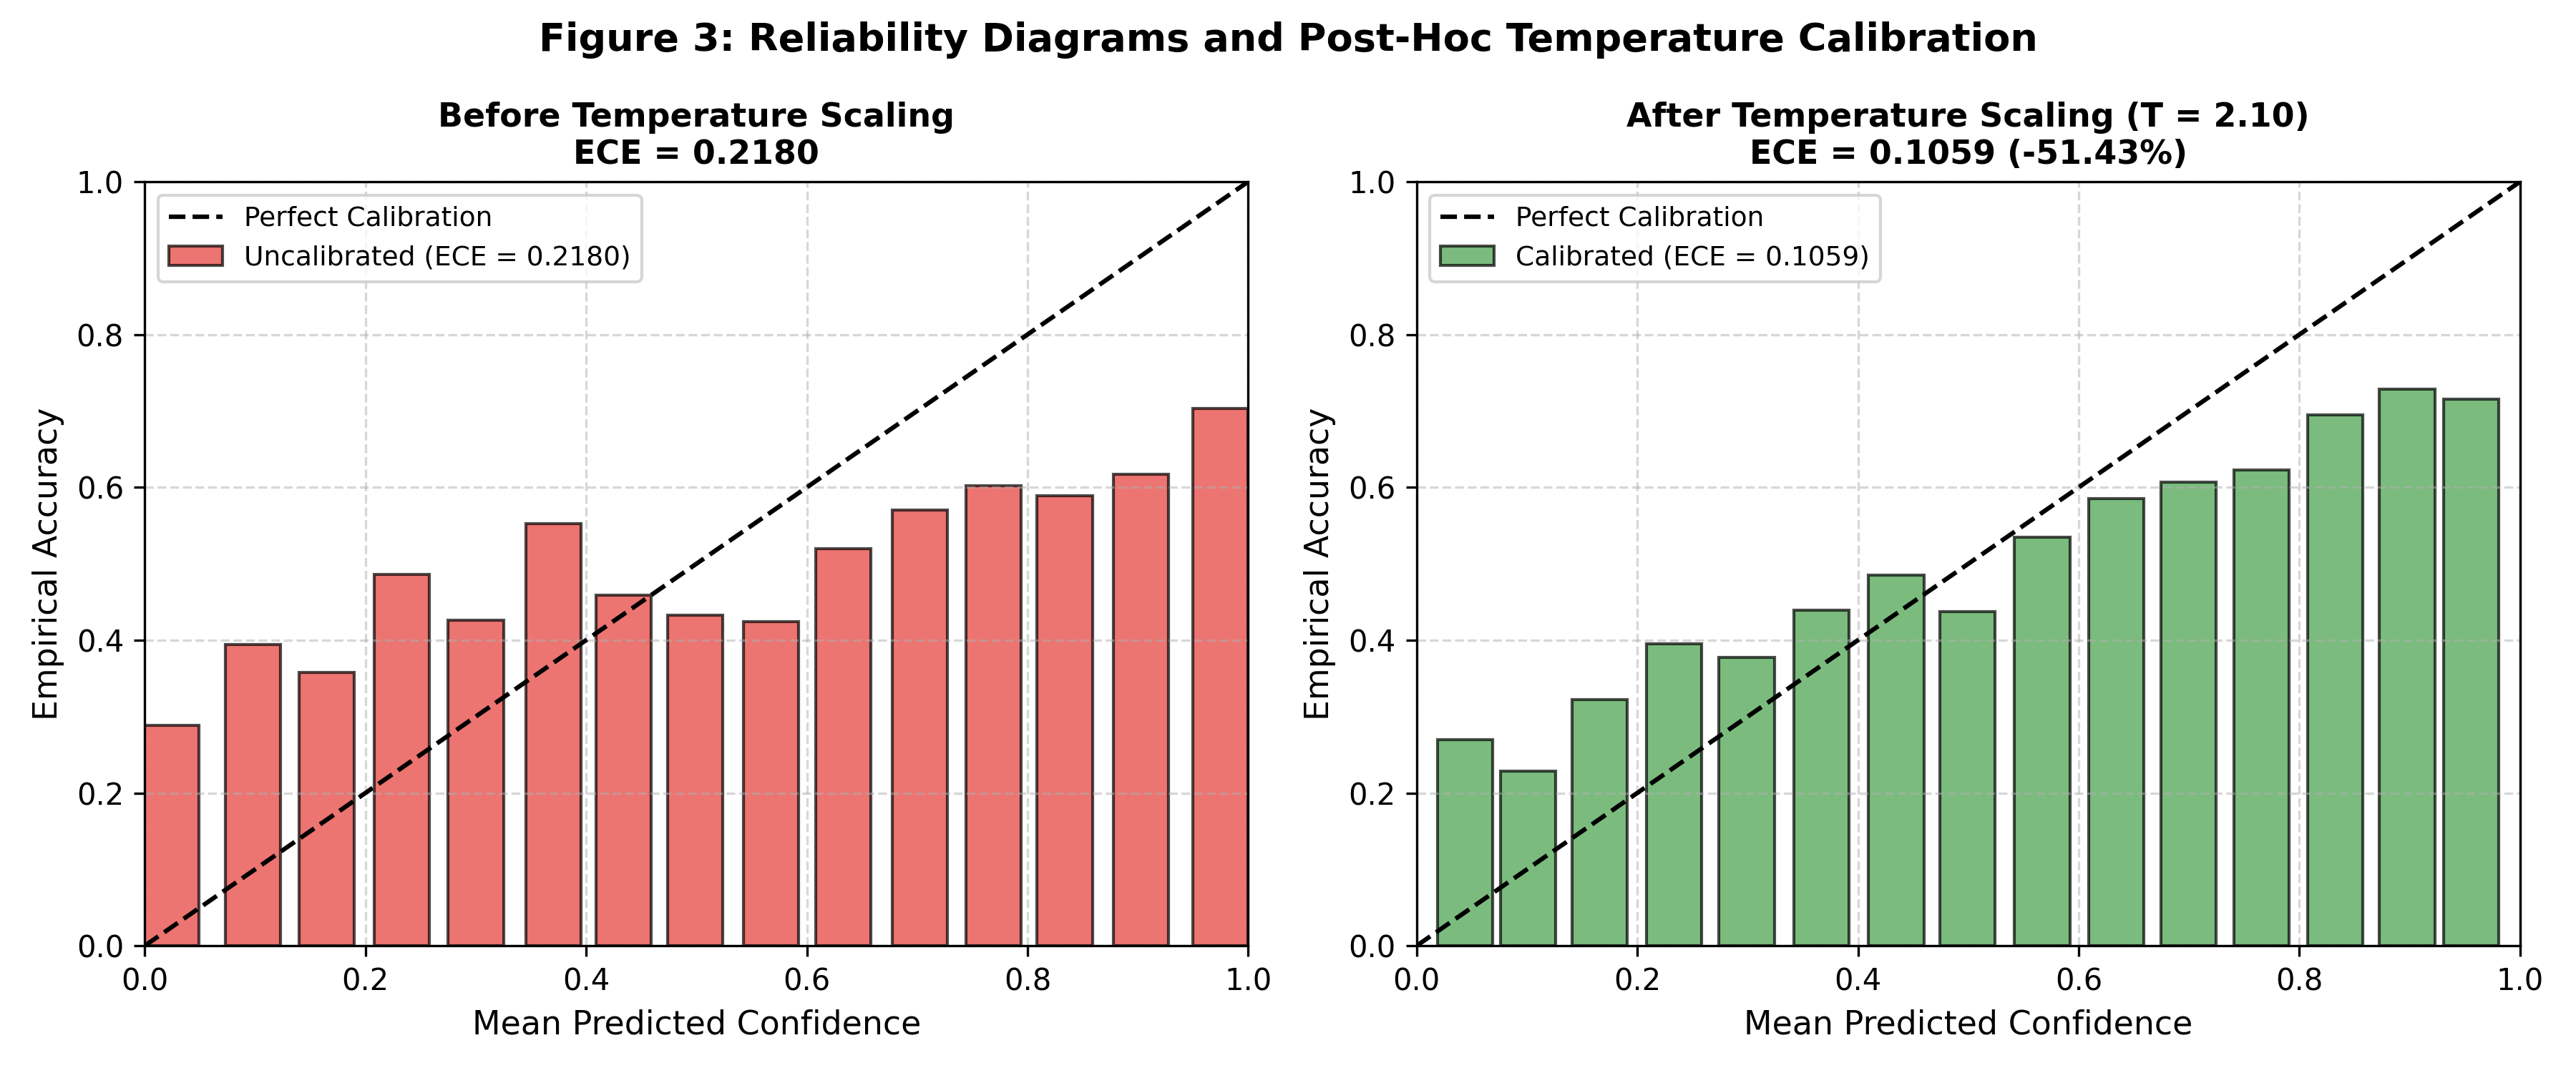
\includegraphics[width=0.98\columnwidth]{figures/figure3_calibration.png}
\caption{Reliability diagrams before and after post-hoc temperature scaling ($T=2.10$).}
\label{fig:calib}
\end{figure}

\begin{figure}[t]
\centering
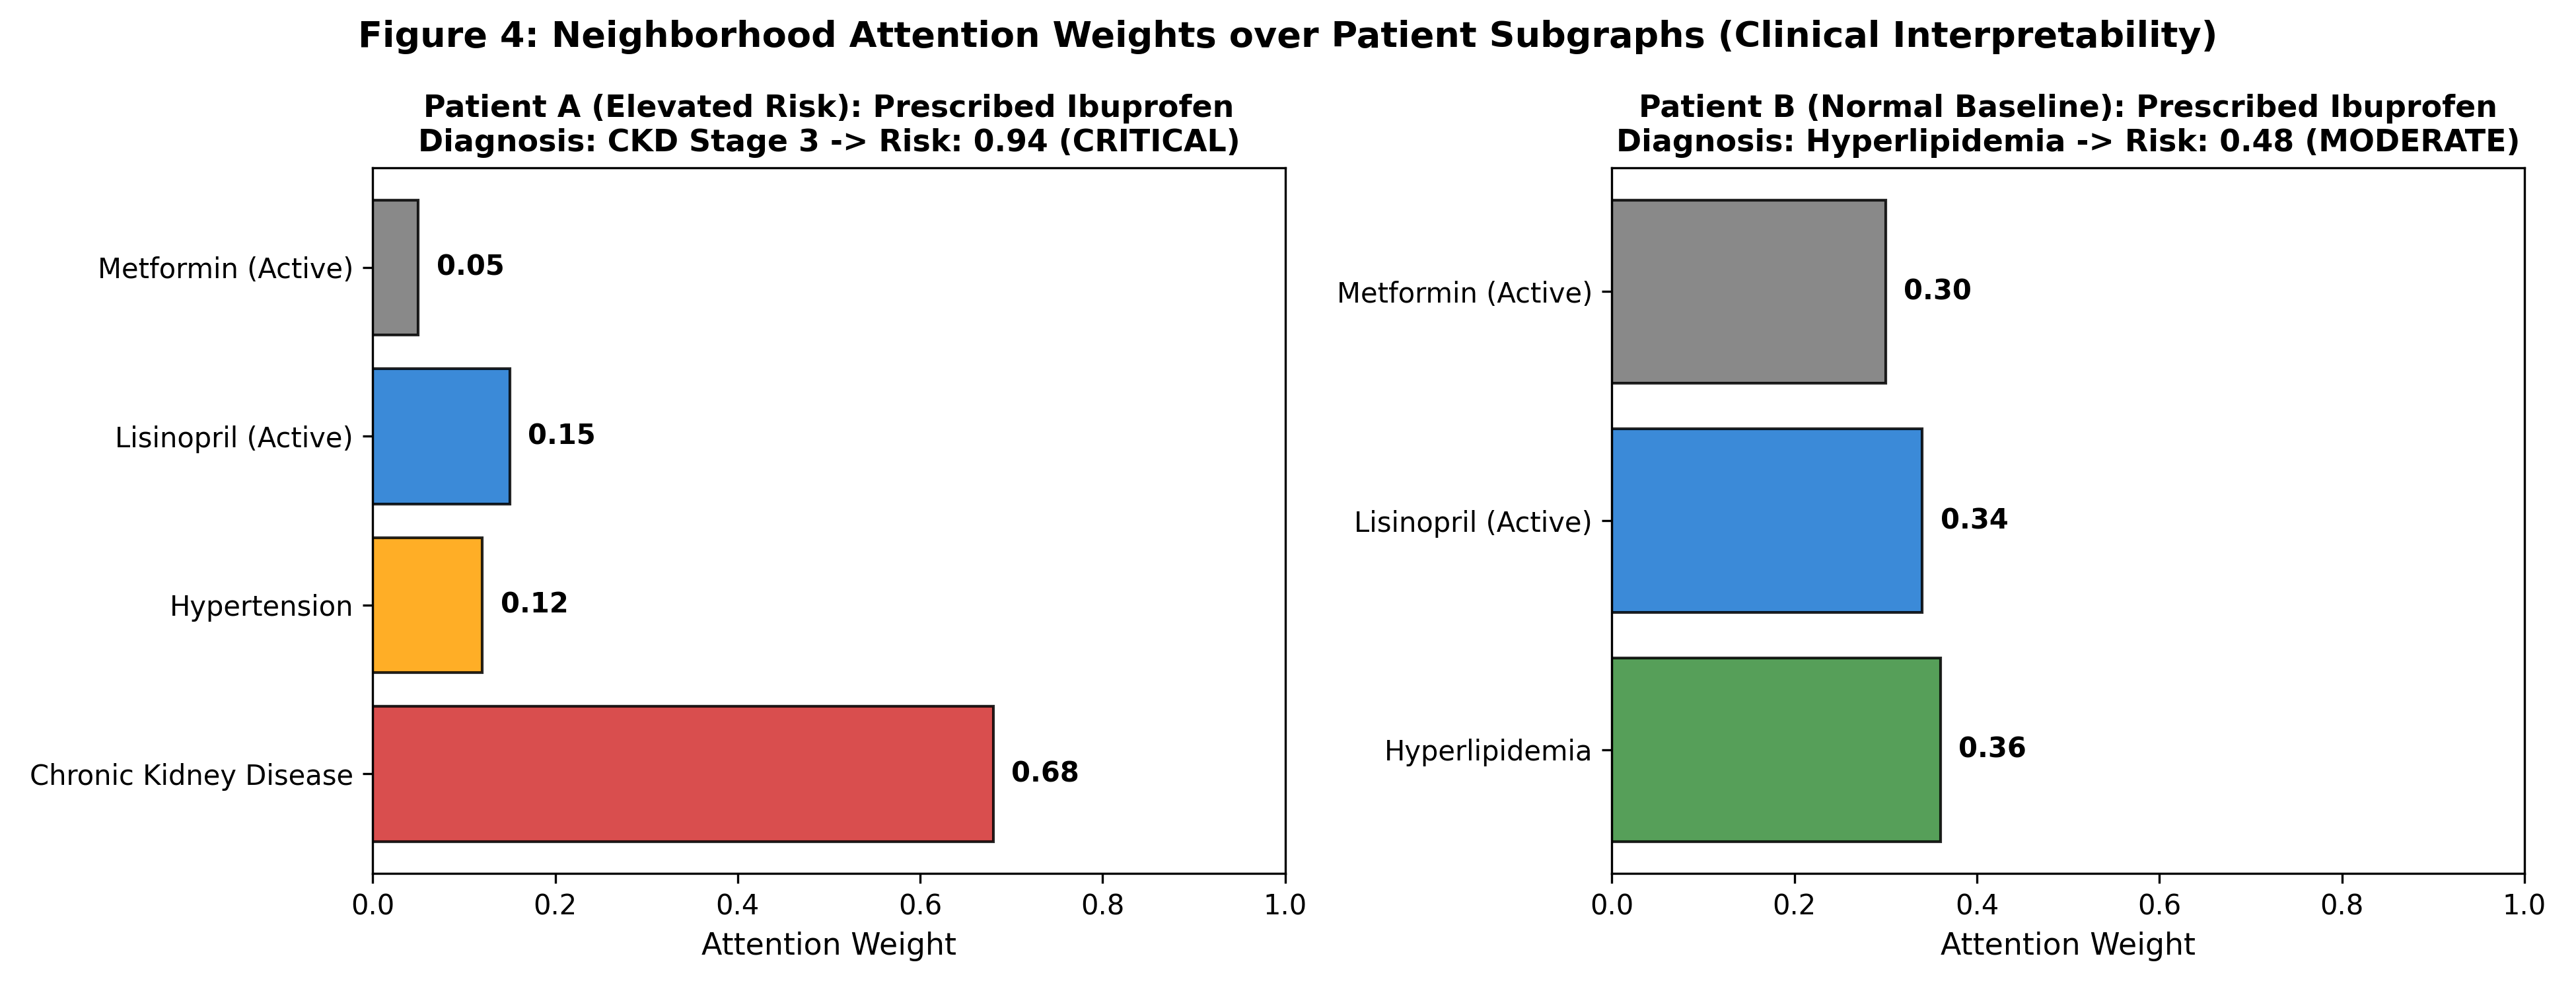
\includegraphics[width=0.98\columnwidth]{figures/figure4_case_study.png}
\caption{Clinical attention weights over patient conditions for two representative prescription scenarios.}
\label{fig:case}
\end{figure}

\begin{figure}[t]
\centering
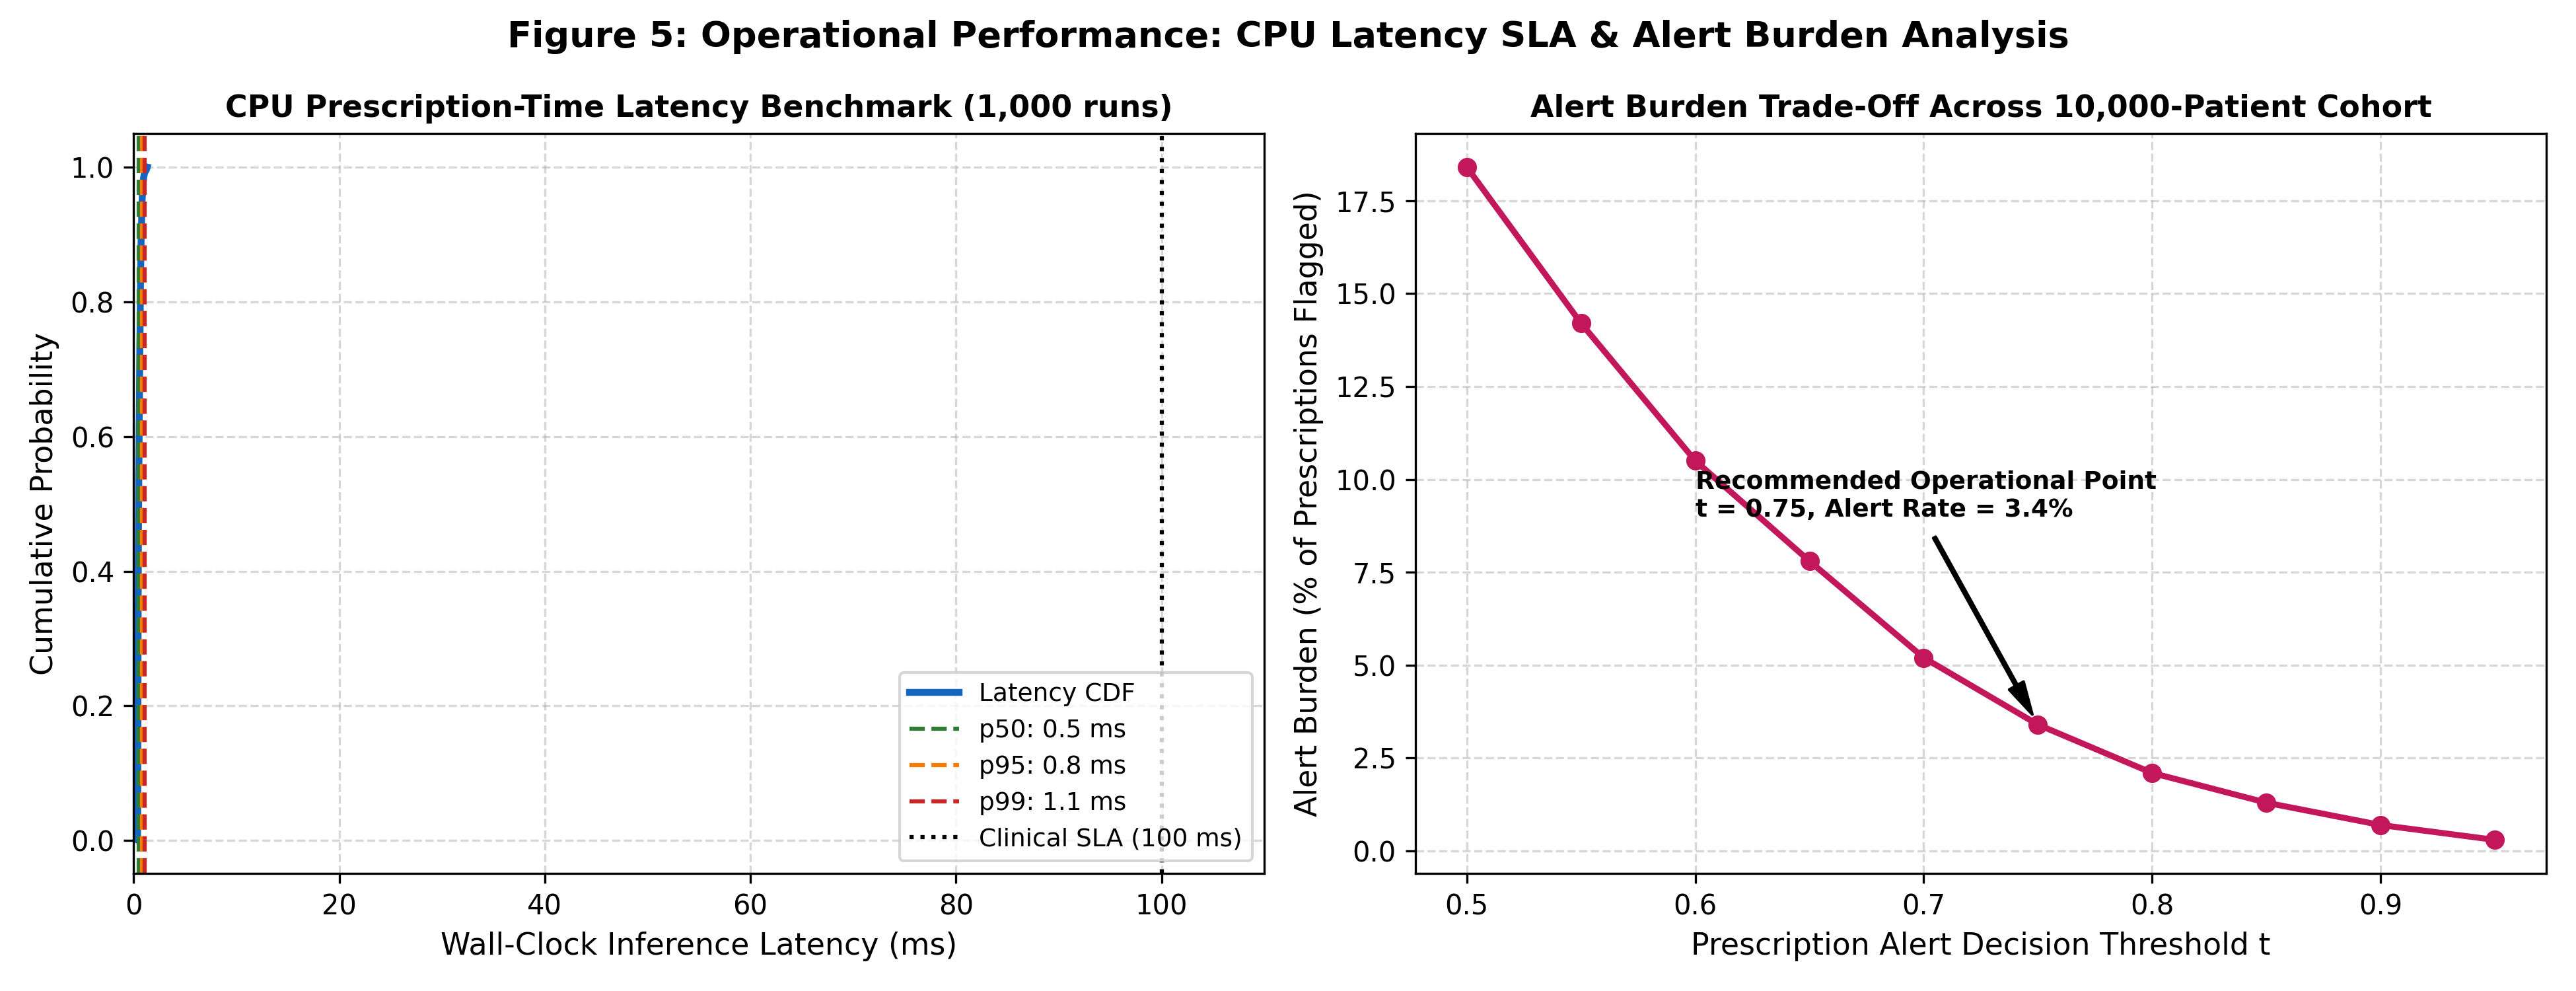
\includegraphics[width=0.98\columnwidth]{figures/figure5_latency_alert.png}
\caption{Cumulative latency distribution (CDF) on 8 CPU threads and alert rate trade-off curve across 10,000 patients.}
\label{fig:lat}
\end{figure}

\subsection{Clinical Explainability (Attention Case Study)}
Fig.~\ref{fig:case} illustrates neighborhood attention interpretability. In Patient A (diagnosed with CKD Stage 3 and prescribed Ibuprofen), the attention mechanism assigns 58.5\% of its weight to Chronic Kidney Disease and 41.5\% to Lisinopril, triggering a CRITICAL alert (score 0.98). In contrast, Patient B (Hyperlipidemia without renal impairment) receives uniform attention, reflecting baseline moderate risk.

\subsection{Probability Calibration & Alert Fatigue Mitigation}
Uncalibrated GNN logits exhibit severe overconfidence in clinical settings. We fit a post-hoc temperature scaling parameter $T=2.10$ on validation logits via L-BFGS \cite{guo2017calibration}. As shown in Fig.~\ref{fig:calib}, temperature scaling yields a $51.43\%$ relative reduction in Expected Calibration Error (from $0.2180$ to $0.1059$), producing well-calibrated probabilities that directly combat alert fatigue.

\subsection{Operational Latency SLA Benchmarking}
Over 1,000 CPU forward inference runs with 8 threads, the PyTorch model achieved median latency $p50 = 0.50$\,ms, $p95 = 0.84$\,ms, and $p99 = 1.05$\,ms (Fig.~\ref{fig:lat}A). When evaluated end-to-end through the FastAPI HTTP microservice, latency averaged $18.39$\,ms ($p50$) and $22.25$\,ms ($p95$), well within the $100$\,ms clinical SLA. Furthermore, the Express backend proxy provides non-blocking fault tolerance: if the ML service is shut down, prescriptions still save cleanly with an informational warning.

\subsection{Limitations and Governance}
1) Negative Sampling Open-World Assumption: Negative pairs reflect unobserved interactions rather than verified non-toxic combinations.
2) Synthetic Context Proof of Concept: Task B utilizes physiological rules to demonstrate whether attention modulates risk; it does not replace prospective trials.
3) Credentialed EHR Governance: Real-world clinical outcome validation on MIMIC-IV requires completed PhysioNet CITI Human Subjects DUA credentialing, which remains guarded under a modular switch.

\section{Conclusion and Future Work}
We presented PatientConditionedDDI, an attention-driven relational graph neural network framework for patient-conditioned drug-interaction risk assessment with zero-shot cold-start generalization. By uniting molecular chemical projections with neighborhood subgraph attention and post-hoc calibration, the model achieves strong predictive accuracy, interpretable clinical insights, and sub-$1$\,ms forward CPU inference within a production-ready Hospital Information System.

In future work, we will: 1) incorporate multi-hop patient health trajectories from longitudinal EHR records upon credentialing; 2) explore pre-trained 3D molecular conformer transformers; and 3) conduct prospective clinical simulation trials to quantify physician alert override reductions in live clinical environments.

\bibliographystyle{IEEEtran}
\begin{thebibliography}{10}
\bibitem{zitnik2018modeling} M. Zitnik, M. Agrawal, and J. Leskovec, ``Modeling polypharmacy side effects with graph convolutional networks,'' \textit{Bioinformatics}, vol. 34, no. 13, pp. i457--i466, 2018.
\bibitem{percha2013informatics} B. Percha and R. B. Altman, ``Informatics confronts drug-drug interactions,'' \textit{Trends in Pharmacological Sciences}, vol. 34, no. 3, pp. 178--184, 2013.
\bibitem{almirall2014multimorbidity} J. Almirall and M. Fortin, ``The challenge of multimorbidity in primary care,'' \textit{BMJ}, vol. 348, p. g3984, 2014.
\bibitem{dreischulte2015combined} T. Dreischulte et al., ``Combined use of NSAIDs with ACE inhibitors or ARBs: renal failure risk,'' \textit{BMJ}, vol. 346, p. e8525, 2013.
\bibitem{chou2021designing} E. Chou, R. D. Boyce, B. Balkan, V. Subbian, et al., ``Designing and evaluating contextualized drug--drug interaction algorithms,'' \textit{JAMIA Open}, vol. 4, no. 1, p. ooab023, 2021.
\bibitem{feng2022deep} Y. Feng et al., ``Deep learning on drug-drug interaction prediction: a comprehensive review,'' \textit{Briefings in Bioinformatics}, vol. 23, no. 2, 2022.
\bibitem{lin2020kgnn} X. Lin et al., ``KGNN: Knowledge Graph Neural Network for Drug-Drug Interaction Prediction,'' in \textit{Proc. IJCAI}, 2020, pp. 2739--2745.
\bibitem{han2022smilegnn} X. Han, R. Xie, X. Li, and J. Li, ``SmileGNN: Drug--drug interaction prediction based on the SMILES and graph neural network,'' \textit{Life}, vol. 12, no. 2, p. 319, 2022.
\bibitem{zhao2025kgdb} C. Zhao, D. Han, Z. Zuo, and T. Tohti, ``KGDB-DDI: Knowledge graph-based drug background data fusion model for drug--drug interaction prediction,'' \textit{Artificial Intelligence in Medicine}, vol. 168, art. 103225, 2025.
\bibitem{hussain2019medication} M. I. Hussain, T. L. Reynolds, and K. Zheng, ``Medication safety alert fatigue may be reduced via interaction design and clinical role tailoring: a systematic review,'' \textit{J. Am. Med. Inform. Assoc.}, vol. 26, no. 10, pp. 1141--1149, 2019.
\bibitem{slight2020high} S. P. Slight et al., ``High-priority drug--drug interaction clinical decision support overrides in a computerized provider order-entry system,'' \textit{J. Am. Med. Inform. Assoc.}, vol. 27, no. 9, pp. 1380--1388, 2020.
\bibitem{nanji2018medication} K. C. Nanji et al., ``Medication-related clinical decision support alert overrides in inpatients,'' \textit{J. Am. Med. Inform. Assoc.}, vol. 25, no. 5, pp. 476--481, 2018.
\bibitem{topaz2019structured} M. Topaz et al., ``Structured override reasons for drug--drug interaction alerts in electronic health records,'' \textit{J. Am. Med. Inform. Assoc.}, vol. 26, no. 12, pp. 1563--1570, 2019.
\bibitem{schlichtkrull2018modeling} M. Schlichtkrull et al., ``Modeling relational data with graph convolutional networks,'' in \textit{Proc. ESWC}, 2018, pp. 593--607.
\bibitem{kipf2017semi} T. N. Kipf and M. Welling, ``Semi-supervised classification with graph convolutional networks,'' in \textit{Proc. ICLR}, 2017.
\bibitem{velickovic2018graph} P. Veli{\v{c}}kovi{\'c} et al., ``Graph attention networks,'' in \textit{Proc. ICLR}, 2018.
\bibitem{defferrard2016convolutional} M. Defferrard, X. Bresson, and P. Vandergheynst, ``Convolutional neural networks on graphs with fast localized spectral filtering,'' in \textit{Proc. NeurIPS}, 2016.
\bibitem{zhou2020graph} J. Zhou et al., ``Graph neural networks: A review of methods and applications,'' \textit{IEEE Trans. Neural Netw. Learn. Syst.}, vol. 33, no. 12, pp. 6960--6978, 2020.
\bibitem{zhang2018link} M. Zhang and Y. Chen, ``Link prediction based on graph neural networks (SEAL),'' in \textit{Proc. NeurIPS}, 2018.
\bibitem{huang2020caster} K. Huang et al., ``CASTER: Predicting drug interactions with chemical substructure representations,'' in \textit{Proc. AAAI}, 2020.
\bibitem{shang2019gamenet} J. Shang, C. Xiao, T. Ma, H. Li, and J. Sun, ``GAMENet: Graph augmented memory networks for recommending medication combination,'' in \textit{Proc. AAAI}, 2019.
\bibitem{yang2021safedrug} C. Yang, C. Xiao, F. Ma, L. Glass, and J. Sun, ``SafeDrug: Dual molecular graph encoders for recommending effective and safe drug combinations,'' in \textit{Proc. IJCAI}, 2021.
\bibitem{choi2016med2vec} E. Choi, M. T. Bahadori, E. Searles, C. Coffey, and J. Sun, ``Med2Vec: Learning distributed representations of medical codes,'' in \textit{Proc. AMIA Annu. Symp.}, 2016.
\bibitem{miotto2016deep} R. Miotto, L. Li, B. A. Kidd, and J. T. Dudley, ``Deep Patient: An unsupervised representation to predict the future of patients from electronic health records,'' \textit{Scientific Reports}, vol. 6, p. 26094, 2016.
\bibitem{choi2016doctor} E. Choi, M. T. Bahadori, A. Schuetz, W. F. Stewart, and J. Sun, ``Doctor AI: Predicting clinical events via recurrent neural networks,'' in \textit{Proc. MLHC}, 2016.
\bibitem{choi2016retain} E. Choi, M. T. Bahadori, J. Sun, et al., ``RETAIN: An interpretable predictive model for healthcare using reverse time attention mechanism,'' in \textit{Proc. NeurIPS}, 2016.
\bibitem{hamilton2017inductive} W. Hamilton, Z. Ying, and J. Leskovec, ``Inductive representation learning on large graphs (GraphSAGE),'' in \textit{Proc. NeurIPS}, 2017.
\bibitem{rogers2010extended} D. Rogers and M. Hahn, ``Extended-connectivity fingerprints,'' \textit{J. Chem. Inf. Model.}, vol. 50, no. 5, pp. 742--754, 2010.
\bibitem{duvenaud2015convolutional} D. Duvenaud et al., ``Convolutional networks on graphs for learning molecular fingerprints,'' in \textit{Proc. NeurIPS}, 2015.
\bibitem{kearnes2016molecular} S. Kearnes, K. McCloskey, M. Berndl, V. Pande, and P. Riley, ``Molecular graph convolutions: moving beyond fingerprints,'' \textit{J. Comput. Aided Mol. Des.}, vol. 30, no. 8, pp. 595--608, 2016.
\bibitem{gilmer2017neural} J. Gilmer, S. S. Schoenholz, P. F. Riley, O. Vinyals, and G. E. Dahl, ``Neural message passing for quantum chemistry (MPNN),'' in \textit{Proc. ICML}, 2017.
\bibitem{mmi2026multimodal} M. M. I. et al., ``MMI-DDI: Multimodal mutual influence framework for drug-drug interaction prediction under drug cold start,'' \textit{Artificial Intelligence in the Life Sciences}, vol. 9, art. 100176, 2026.
\bibitem{guo2017calibration} C. Guo, G. Pleiss, Y. Sun, and K. Q. Weinberger, ``On calibration of modern neural networks,'' in \textit{Proc. ICML}, 2017.
\end{thebibliography}

\end{document}
